%\VignetteIndexEntry{Statistical Working Paper on balancing of the FBS}
%\VignetteEngine{knitr::knitr}
\documentclass[nojss]{jss}\usepackage[]{graphicx}\usepackage[]{color}
%% maxwidth is the original width if it is less than linewidth
%% otherwise use linewidth (to make sure the graphics do not exceed the margin)
\makeatletter
\def\maxwidth{ %
  \ifdim\Gin@nat@width>\linewidth
    \linewidth
  \else
    \Gin@nat@width
  \fi
}
\makeatother

\definecolor{fgcolor}{rgb}{0.345, 0.345, 0.345}
\newcommand{\hlnum}[1]{\textcolor[rgb]{0.686,0.059,0.569}{#1}}%
\newcommand{\hlstr}[1]{\textcolor[rgb]{0.192,0.494,0.8}{#1}}%
\newcommand{\hlcom}[1]{\textcolor[rgb]{0.678,0.584,0.686}{\textit{#1}}}%
\newcommand{\hlopt}[1]{\textcolor[rgb]{0,0,0}{#1}}%
\newcommand{\hlstd}[1]{\textcolor[rgb]{0.345,0.345,0.345}{#1}}%
\newcommand{\hlkwa}[1]{\textcolor[rgb]{0.161,0.373,0.58}{\textbf{#1}}}%
\newcommand{\hlkwb}[1]{\textcolor[rgb]{0.69,0.353,0.396}{#1}}%
\newcommand{\hlkwc}[1]{\textcolor[rgb]{0.333,0.667,0.333}{#1}}%
\newcommand{\hlkwd}[1]{\textcolor[rgb]{0.737,0.353,0.396}{\textbf{#1}}}%

\usepackage{framed}
\makeatletter
\newenvironment{kframe}{%
 \def\at@end@of@kframe{}%
 \ifinner\ifhmode%
  \def\at@end@of@kframe{\end{minipage}}%
  \begin{minipage}{\columnwidth}%
 \fi\fi%
 \def\FrameCommand##1{\hskip\@totalleftmargin \hskip-\fboxsep
 \colorbox{shadecolor}{##1}\hskip-\fboxsep
     % There is no \\@totalrightmargin, so:
     \hskip-\linewidth \hskip-\@totalleftmargin \hskip\columnwidth}%
 \MakeFramed {\advance\hsize-\width
   \@totalleftmargin\z@ \linewidth\hsize
   \@setminipage}}%
 {\par\unskip\endMakeFramed%
 \at@end@of@kframe}
\makeatother

\definecolor{shadecolor}{rgb}{.97, .97, .97}
\definecolor{messagecolor}{rgb}{0, 0, 0}
\definecolor{warningcolor}{rgb}{1, 0, 1}
\definecolor{errorcolor}{rgb}{1, 0, 0}
\newenvironment{knitrout}{}{} % an empty environment to be redefined in TeX

\usepackage{alltt}
\usepackage{url}
\usepackage[sc]{mathpazo}
\usepackage{geometry}
\geometry{verbose,tmargin=2.5cm,bmargin=2.5cm,lmargin=2.5cm,rmargin=2.5cm}
\setcounter{secnumdepth}{2}
\setcounter{tocdepth}{2}
\usepackage{breakurl}
\usepackage{hyperref}
\usepackage[ruled, vlined]{algorithm2e}
\usepackage{mathtools}
\usepackage{draftwatermark}
\usepackage{float}
\usepackage{placeins}
\usepackage{mathrsfs}
\usepackage{multirow}
%% \usepackage{mathbbm}
\DeclareMathOperator{\sgn}{sgn}
\DeclareMathOperator*{\argmax}{\arg\!\max}







\title{\bf Statistical Working Paper on Balancing Methodology for
 Food Balance Sheet (FBS)}

\author{Marco Garieri, Natalia Golini, Luca Pozzi \\ Food and Agriculture Organization \\ of
  the United Nations}

\Plainauthor{M. Garieri, N. Golini, L. Pozzi} 

\Plaintitle{Statistical Working Paper on Imputation Methodology for
  the FAOSTAT Production Domain}

\Shorttitle{Balancing FBS}

\Abstract{ 

\noindent 
In this paper we describe a sampling strategy to generate balanced FBSs. 
 A FBS is a collection of information from different sources (official and unofficial) 
 prone to measures errors and uncertainties. Our method tries to solve the 
 problem of  balancing the FBSs in a flexible way, trusting reliable information 
 and re-allocating the uncertainty over the non-reliable information. Considering 
 agro-economical information in the form of minimal constrains and objective functions, 
 we are able to produce a unique solution (balanced FBS).
}

\Keywords{Food Balance Sheet, FBS, Balancing, Structural Zero}
\Plainkeywords{Food Balance Sheet, FBS, Balancing, Structural Zero}

\Address{
  Marco Garieri, Natalia Golini, Luca Pozzi\\
  Economics and Social Statistics Division (ESS)\\
  Economic and Social Development Department (ES)\\
  Food and Agriculture Organization of the United Nations (FAO)\\
  Viale delle Terme di Caracalla 00153 Rome, Italy\\
  E-mail: \email{marco.garieri@fao.org}\\
  URL: \url{https://github.com/mrpozzi/conSTable/tree/develop}
}
\IfFileExists{upquote.sty}{\usepackage{upquote}}{}

\begin{document}

\section*{Disclaimer}
This Working Paper should not be reported as representing the official view of
the FAO. The views expressed in this Working Paper are those of the
author and do not necessarily represent those of the FAO or FAO
policy. Working Papers describe research in progress by the authors and
are published to elicit comments and to further discussion.\\

This paper is dynamically generated on \today{} and is subject to
changes and updates.

\section{Introduction}
The Food Balance Sheet presents the overall description of the food supply 
and utilization for a specific country in a defined time period. The information 
provided by the FBSs can be used to analyze the agro-economical 
condition of a country, in particular to assess food security trends over time 
for specific regions \cite{fao2013}. Due to the importance of this information,
FBSs must be precise and reliable.\\

FBSs represent the total food supply and utilization for a specific country in a 
specific year. Unfortunately, as described in "Food Balance Sheets: A handbook" 
\cite{fao2011}, very often the quality and coverage of data is not optimal, varying 
considerably from country to country. 
FBSs are assembled from a variety of sources, official or unofficial, and inaccuracies 
and errors may also be introduced at every level. In case of non-reliable information
 the data are often estimated or adjusted while, in case of missing value, imputed.
As a result, the FBSs are unbalanced, i.e., for each commodity in a specified 
country of the reference period the Total Supply (TS) is not equal to the Total 
Utilization (TU). Then, the balancing of FBSs is a primary problem within FAO.\\

In this paper we introduce a very flexible algorithm to solve the problem of 
balancing FBSs through sampling steps.  The method proposed respects the 
balance equation for each rows (as explain in Section 2) and takes in 
consideration of possible constrains, meaningful from a agro-economical 
point of view, and choose a unique solution that optimizes an appropriate objective function. 
The approach considers all prior information on measurement or estimate 
uncertainties available, in the form of mean and variability around the mean 
($\pm$ sd) per cell or columns, in case only little information is available.\\
 
The paper is structured as follows. Section 2 gives an overview of existing methods,
section 3  describes the FBSs and the 
 methods used to estimate its components. Section 4 shows an the new 
 method to balance the FBSs. Section 5 presents a case study and the 
 conclusions are in Section 6.

\FloatBarrier
\section{Background and Review of Literature}

The balancing problem is well-known in economics literature. Often 
census-based Input-Output (IO) tables or social-accounting matrixes (SAM) are 
cases of not balanced tables. 
Some of the most used approach are the Generalized Maximum Entropy (GME) 
 and the  Generalized Cross Entropy (GCE) techniques \cite{Robinson2000}, \cite{Britz2002},
 \cite{Robilliard2003}. In \cite{Robinson2000}, the 
 authors present a flexible "cross entropy" approach to estimate consistent SAMs 
 starting from data estimated with errors. In this approach the error is a weighed average
 of known constants. Assumption on the weight, considered as prior, has to be given.
 However, in GME and GCE techniques, the interpretation of the prior information 
 remains an unsolved problem. For this reason bayesian approaches have been 
 proposed to overcome to this problem. In a Bayesian framework the prior information 
 held by the researcher has a direct and interpretable formulation \cite{Heckelei2008}, 
 \cite{Rodrigues2014}. However, in this case, a considerable amount of prior 
 information, not available to us, is necessary in order to have a unique solution.


The balancing problem has been associated with the solution of the contingency 
tables  problem with fixed margins, trying to input individual cell entries and inferring 
the model's parameters underlying the table (see \cite{Dinwoodie2011}, \cite{Chen2007}
\cite{Chen2005}, \cite{Dobra2006}, \cite{Tebaldi1998}). In \cite{Dinwoodie2011}, the  
authors propose a combination of a sequential importance sampling (SIS) with a 
sequentially updated normal  proposal distribution. And thus, the maximum entropy 
distribution is sequentially approximated. The algorithm, has to sample all the 
cell conditionally to the constrains,  for this reason is very memory demanding 
and the speed depends on the table dimension. For these reason, and for the 
assumption of non-negative cell value, the method is not suitable for our problem 
of balancing FBSs.



\section{FBS structure}

As mention before, a FBS represents the TU and the TS of food for a given country 
in a specified period. Every row is a single (or aggregated) commodity and every 
column is each element of the Domestic Supply (Production, Imports, Exports and 
Stock Changes) and the Domestic Utilization (Food, Food Manufacture, Feed, 
Seed, Waste, and Other Uses). Each cell is a value expressed in thousands of 
metric tons (see \url{http://faostat3.fao.org/download/FB/FBS/E}).\\
In Figure \ref{tab:fbs_italy_2011}, the first lines of the FBS for Italy in 2011 are presented. 

%\begin{figure}[!ht]
%  \centering
%%  \includegraphics[scale = 0.7]{figure/dietterich.png}
%\end{figure}


%\begin{knitrout}
%\definecolor{shadecolor}{rgb}{0.969, 0.969, 0.969}\color{fgcolor}\begin{figure}[!ht]

%
%%{\centering \includegraphics[width=\maxwidth]{figure/wheat-yield-explore} 

%}


\begin{knitrout}
%\definecolor{shadecolor}{rgb}{0, 0, 0}\color{fgcolor}
\begin{figure}[!ht]
{\centering 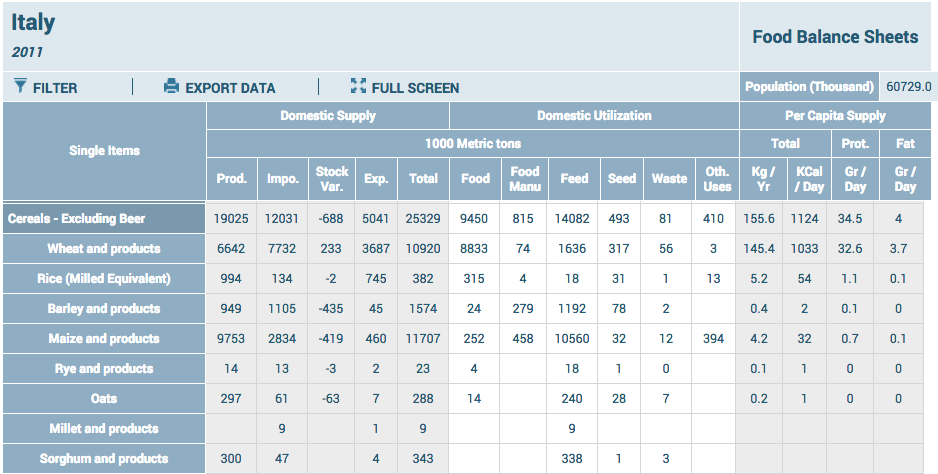
\includegraphics[width=\maxwidth]{figure/fbs_italy_2011.png} 
}
\caption[First lines of the FBS for Italy in 2011.]{First lines of the FBS for Italy in 2011.
\label{tab:fbs_italy_2011}}

\end{figure}
\end{knitrout}

\subsection{Balancing equation}
The term "balancing table" refers to the attempt to balance accounts 
in each country for each commodity. This is done by matching supply (Production, 
Imports, Stock Changes and Exports) and uses (Food, Food Manufacturing, 
Feed, Seed, Waste,  and Other Uses).\\
For each commodity $i$ in a given country $c$ at time $t$ the Total Supply 
(TU) and the Total Domestic Utilization (TU) are described as following: 

\begin{align*}
	{\text TS}_{c,t,i} &= {\text Production}_{c,t,i} + {\text Imports}_{c,t,i} 
	+ {\text StockVar}_{c,t,i} - {\text Exports}_{c,t,i}\\
	{\text TU}_{c,t,i} & = {\text Food}_{c,t,i} + {\text FoodManu}_{c,t,i} 
	+ {\text Feed}_{c,t,i} + {\text Seed}_{c,t,i} + {\text Waste}_{c,t,i} 
	+ {\text OtherUses}_{c,t,i}
\end{align*}

Where with ${\text StockVar}_{c,t,i}$ we consider the difference between 
the level of stock at time $t$ and time $t-1$. In order to have a "balanced" 
or "closed" FBS the following balance identity needs to hold:

\begin{equation}\label{eq}
{\text TS}_{c,t,i} = {\text TU}_{c,t,i} \quad\quad \forall i
\end{equation}

The identity \ref{eq} is often not respected, due to the uncertainty of data, 
as explained in the previous section, Mahjoubi and Prakash (2012) and 
FAO (2014)

\subsection{Methods for  estimate TS and TU}
Apart from Production and trade (Imports and Exports), which are collected 
through questionnaires, all  other elements of the FBS are usually estimated 
and official data are available only for very few developed countries 
\cite{Mahjoubi2012}, \cite{fao2014}.

\subsubsection{Production and trade}
Due to these elements' reliability they drive the FBS production system. 
Consequently, data collection efforts, especially in the Production domain, that 
rely on questionnaire response, remain key. The information that FBS supplies 
ultimately can only be as good as the core underlying data, and concerted action 
is required to improve data inflows.\\

More can be said about Production imputation, reference Michael's paper.

\subsubsection{Food}
This term represents the total supply of all agricultural and derived products 
available for human consumption. Food available can be reported in terms of 
primary product equivalent such as wheat and milk or in the form that the products 
may actually be consumed, such as bread and cheese. This number is typically 
the residual of the balance sheet. However, due to uncertainty surrounding many 
other elements of the balance and because of weak methods and outdated 
parameters, food is not the only residual element. In order to have an accurate 
estimate for food measurement  a methodological framework for incorporating 
information from other existing statistical sources of information, i.e. Nationally 
representative Household Survey (NHS) is under development. \\

Jim work. Reference as soon as available.

\subsubsection{Food Processing}
This term, also known as Food Manufacturing, is the amount of a commodity 
processed for food purposes and for which separate entries are provided in the 
FBSs either in the same commodity tree or in another food commodity. This 
helps to maintain the concept of accounting for all foods (once and only once) 
and maintains the links in the various levels of the balance sheets.

\subsubsection{Feed}
This term represents the quantity of the commodity available for feeding to 
livestock and poultry during the year. Less than 15\% of the countries respond 
to FAO's feed questionnaire and most of them are developed countries. For the 
rest of the world, a new method was developed. It is divided in two steps: 
\begin{itemize}
\item[i] determine feed requirements for metabolizable energy and protein 
\item[ii] determine allocation of compound/concentrate feedstuffs to match 
requirements. 
\end{itemize}

See FAO (2014) for more details, and reference Onno work.

\subsubsection{Seed}
Among the different categories of utilization, Seed use is one of the few categories 
which can be modeled a priori according to a deterministic rule, animal feed is 
possibly another. Seeding rates, and ultimately the demand for seed, can be modeled 
as a function of target plant density, establishment percentage, and seed weight. 
Multiplied by area planted, seed use can then be derived. However, with the rise 
in high-precision commercial farming, many farmers are choosing to use certified 
seed, purchased from specialized seed farmers. This trend requires the need to 
capture commercial seed production quantities.\\

Reference Josh work. 

\subsubsection{Waste}
This term is the amount of the commodity lost through wastage during the year 
at all stages between farms and the household level in handling, storage and transport, 
but not including waste in the edible and inedible part of the commodity which occurs 
after the commodity has entered the household. The quantities lost during processing 
are also not included under this element because they are implicitly considered in applying 
the underlying extraction rate. Waste data have been reviewed for some 140 developing 
countries. It can be seen that the coefficients developed to calculate waste in FAOSTAT 
(waste is calculated as a percentage of total supply) have been constant for many years. 
Moreover, the review shows inconsistencies in the waste parameters among countries, 
and commodities within countries.\\

Reference Klaus work.

\subsubsection{Other Utilization}
This term is a miscellaneous category to account for all other uses not identified 
elsewhere (e.g. the use of maize to produce ethanol). This category also includes 
consumption by those who are not accounted in the country's population 
(e. g., tourists).\\

Reference Jim work on tourism. 

\subsubsection{Stock Changes}
Limited information exists on opening or closing stocks for many commodities in 
many countries, making stocks estimation complicated and imprecise. As a result, 
stock changes are often calculated to smooth supply and utilization. In practice, 
they are used as a balancing factor and they may, in part, be calculated residually 
by first estimating food available for consumption. As the item is partially and 
residually derived it then reflects not only stock changes but also other statistical 
errors in the food balance equation.

\section{An alternative approach to balance FBSs}
\subsection{Problem formulation}
A generale FBS looks like the following


\begin{table}[h!]
  \label{tab:example}
  \caption{Scheme of the FBS}
  \begin{center}
    \begin{tabular}{|c||c|c|c|c|c|c||c|}
      \hline
       & $L_1$&$L_2$&$\dots$&$L_j$&$\dots$&$L_s$&$Tot Rows$\\
       \hline\hline
       $C_1$ & $x_{11}$&$x_{12}$&$\dots$&$x_{1j}$&$\dots$&$x_{1s}$&$R_1$\\
       \hline
        $C_2$ & $x_{21}$&$x_{22}$&$\dots$&$x_{2j}$&$\dots$&$x_{2s}$&$R_2$\\
        \hline
        $\dots$ & $\dots$&$\dots$&$\dots$&$\dots$&$\dots$&$\dots$&$\dots$\\
        \hline
        $C_i$ & $x_{i1}$&$x_{i2}$&$\dots$&$x_{ij}$&$\dots$&$x_{is}$&$R_i$\\
        \hline
        $\dots$ & $\dots$&$\dots$&$\dots$&$\dots$&$\dots$&$\dots$&$\dots$\\
        \hline
        $C_r$ & $x_{r1}$&$x_{r2}$&$\dots$&$x_{rj}$&$\dots$&$x_{rs}$&$R_r$\\
        \hline\hline
        $Tot Cols$ & $T_{1}$&$T_{2}$&$\dots$&$T_{j}$&$\dots$&$T_{s}$&Tot\\
      \hline
    \end{tabular}
  \end{center}  
\end{table}

Each row $C_i$ represents a commodity and each column $L_j$ represents 
a level, both supply or utilization.  The table satisfies the following identities:

\begin{align}
	R_i &= \sum_{j=1}^{s}x_{ij}\\
	T_j & = \sum_{i=1}^{r}x_{ij}\\
	Tot & = \sum_{i=1}^{r} R_i = \sum_{j=1}^{s} T_j = \sum_{i=1}^{r}\sum_{j=1}^{s}x_{ij}
\end{align}	

First of all, we assume that for each commodity $C_i$, its total row  $R_i$ is fixed. 
This means that we rearrange the balancing identity shown in \ref{eq} placing to 
the left of the equation the terms that come from official sources, hereafter called 
consolidated terms, and to right those coming from unofficial sources. In our 
example, Production is the only consolidated term. Then, the balancing identity
 \ref{eq} can be rewritten in the following way:

\begin{align*}
	{\text Production}_{c,t,i} = & - {\text Imports}_{c,t,i} - {\text StockVar}_{c,t,i} + 
	{\text Exports}_{c,t,i} \\
	 & + {\text Food}_{c,t,i} + {\text FoodManu}_{c,t,i} 
	+ {\text Feed}_{c,t,i} + {\text Seed}_{c,t,i} + {\text Waste}_{c,t,i} 
	+ {\text OtherUses}_{c,t,i}
\end{align*}	

where ${\text StockVar}_{c,t,i} = {\text Stock}_{c,t,i} - {\text Stock}_{c,t-1,i}$. Then the FBS assumes the form of the following table:

\begin{table}[h!]
  \label{tab:fbstab}
  \caption{Scheme of the FBS}
  \begin{center}
    \begin{tabular}{|c||c|c|c|c|c|c|c|c|c||c|}
      \hline
       & Imps&StockV&Exps&Food&FoodM&Feed&Seed&Waste&Other&Production\\
       \hline\hline
       $C_1$ & $x_{11}$ & $x_{12}$ & $x_{13}$ & $x_{14}$ & $x_{15}$ & $x_{16}$ & $x_{17}$ & $x_{18}$ & $x_{19}$ & $R_{1}$\\
       \hline
       $C_2$ & $x_{21}$ & $x_{22}$ & $x_{23}$ & $x_{24}$ & $x_{25}$ & $x_{26}$ & $x_{27}$ & $x_{28}$ & $x_{29}$ & $R_{2}$\\
       \hline
        $\dots$ & $\dots$ & $\dots$ & $\dots$ & $\dots$ & $\dots$ & $\dots$ & $\dots$ & $\dots$ & $\dots$ & $\dots$\\
        \hline
       $C_i$ & $x_{i1}$ & $x_{i2}$ & $x_{i3}$ & $x_{i4}$ & $x_{i5}$ & $x_{i6}$ & $x_{i7}$ & $x_{i8}$ & $x_{i9}$ & $R_{i}$\\
       \hline
        $\dots$ & $\dots$ & $\dots$ & $\dots$ & $\dots$ & $\dots$ & $\dots$ & $\dots$ & $\dots$ & $\dots$ & $\dots$\\
        \hline
       $C_r$ & $x_{r1}$ & $x_{r2}$ & $x_{r3}$ & $x_{r4}$ & $x_{r5}$ & $x_{r6}$ & $x_{r7}$ & $x_{r8}$ & $x_{r9}$ & $R_{r}$\\
        \hline\hline
        $Tot Cols$ & $T_{1}$&$T_{2}$&$T_{3}$&$T_{4}$&$T_{5}$&$T_{6}$&$T_{7}$&$T_{8}$&$T_{9}$&Tot\\
      \hline
    \end{tabular}
  \end{center}  
\end{table}

In the same way, if we believe that the consolidates terms are more than one, i.e. Production and trade (Imports and Exports), the balancing identity can be rewritten as follows:

\begin{align*}
	{\text Production}_{c,t,i} + {\text Imports}_{c,t,i} - {\text Exports}_{c,t,i} & =  {\text StockVar}_{c,t,i} + {\text Food}_{c,t,i}\\
	 & + {\text FoodManu}_{c,t,i} + {\text Feed}_{c,t,i} + {\text Seed}_{c,t,i} \\
	 & + {\text Waste}_{c,t,i} + {\text OtherUses}_{c,t,i}
\end{align*}	


In this way, we consider data from official sources as highly accurate and reliable data, 
while those from non-official sources prone to potential measurement errors. 
The latter are often estimated or adjusted with a certain degree of error that depends 
on differing concepts, definitions, and methodologies involved in data gathering and 
generation among countries \cite{Jacobs2002}. For these reasons, the 
consolidated terms may change from country to country, and from year to year. \\
Then, we assume that all amounts  $x_{ij}$ are measured with an additive error:
\begin{equation}
y_{ij}= x_{ij}+e_{ij} \quad\quad    \forall i,j
\end{equation}

where $y_{ij}$ represents the commodity value and $e_{ij}$ is the difference 
between the measured value and its real value.\\
As discussed in \cite{Robinson2000}, the classical assumptions made in 
regression analysis ${\text Cov}(x_{ij},e_{ij})=0$ with $e_{ij}\sim  \mathscr{N}
(0,\sigma^2 )~~\forall i,j$ are extremely constraining when little is known about 
the error of structure and data are scarse.
Even if a normal distribution can be attributed to $e_{ij}$, the assumption of zero mean 
seems not realistic in our case.\\
To take into account the measurement error of the individual cells ($x_{ij}$), we assume 
for these values a Normal truncated distribution:
\begin{equation}
x_{ij} \sim TN (\mu_{ij},\sigma_{ij}^2)
\end{equation}

where $\mu_{ij}$ are the estimates for the elements of the TS and TU and $\sigma_{ij}$
is the standard deviation reflecting the degree of uncertainty of the estimates. 

The shape of the distribution will change depending on the prior information available: 
for accurate values the distribution will be narrow, while for not well measured values 
we will have a uniform-like prior. Moreover we have values null with certainty (structural
zeros), i.e., quantities of processed seed use are not measured in the amount of eggs.
Since, each column totals $T_j$ is not a fixed value, the experts can give the possible range
 of outcomes as the interval  $(t_{j,min},t_{j,max})$.  
Since the only fixed values are the rows' totals, the algorithm work independently row by row, 
sampling each cell from its prior distribution. The last value in the row, $x_{is}$, is calculated
as follows:
\begin{equation}
x_{is} = R_i \sum_{j=1}^{s-1} x_{ij}
\end{equation}
If $x_{is}$ falls inside its possible range is accepted, otherwise the row is sampled again.
In this way the computation time is indeed reduced all the uncertainty is shared between 
the less reliable estimates. If the all rows are balanced, the algorithm check the columns' 
totals, and if they fall within each own range. In this case the table is accepted as a possible
solution. 
In all the space of possible tables, an objective function allow to determine the unique solution
to the problem, maximizing or minimizing specific column (or columns) or reducing the variability
from the input table. Different objective functions, and combination of them, can be implemented
in the algorithm, in order to have a table meaningful from the agro-economical prospective.
Other types of constrains can be applied, for example small differences in the short run for the 
same country, but we want to remind the future user that, in case of multiple constrains and objective
functions, the space of possible solution will decrease dramatically.


\section{Case study: Italy 2011}
In this section we present the results obtained by applying this new method to the FBS of 
 Italy in 2011.\\
In this case, the consolidated term is Production (information taken from  FAO experts). So
the balancing equation is the following:

\begin{align*}
	{\text Production}_{Italy,2011,i} = & - {\text Imports}_{Italy,2011,i} - {\text StockVar}_{Italy,2011,i} + 
	{\text Exports}_{Italy,2011t,i} \\
	 & + {\text Food}_{Italy,2011,i} +  {\text Feed}_{Italy,2011,i} + {\text Seed}_{Italy,2011,i} + {\text Losses}_{Italy,2011,i} \\
	& + {\text IndUses}_{Italy,2011,i}
\end{align*}	

where $ {\text StockVar}_{Italy,2011,i} =  {\text Stock}_{Italy,2011,i} - {\text Stock}_{Italy,2010,i}$

Since we present a case of the previous FBS format, FoodManu is missing and Waste is 
replaced by Losses and OtherUses by IndUses. These are the description of the old categories:

\subsubsection{Industrial use}
Agriculture plays an increasingly important role in the industrial economy, providing 
feedstocks for the production of liquid fuels, chemicals and advanced materials, such 
as composites for industry, while the emergence of green industries expands opportunities 
for the rural sector. A generalized model provides reliable estimates of industrial usage. 
Important drivers of industrial usage likely include income, the level of industrialization, 
policy mandates, and a country's comparative advantage in cultivating and processing 
the crop. A data collection strategies that inform other important industrial activities 
involving food crops, such as the Aglink-Cosimo framework of the OECD/FAO, is used t
o test and refine the model.

\subsubsection{Losses}
In the accounts of FBS, food losses are considered to be the amount of lost commodities, 
starting from the moment when production is recorded until it reaches the consumer. 
Food wasted at the household level is not considered as a loss in the FBS, but rather 
as "waste". The FBS reports food losses for each relevant type of food, each country 
and for each year. However, the amount of food loss is not asked in the country's production 
questionnaire and empirical data on food losses are rare. Using "measured" FBS data, 
together with data from additional surveys, loss ratios is imputed for cases in which no 
measured data are available (see \cite{Klaus2014} for more details).\\

In the next table the FBS for Italy 2011 is presented partially. The value are expressed in 
 kilocalories per capita per day (kcal/cap/day), and the structural zeros are presented as 0*.
(In this case StockVar was calculated as a difference from the other values, thus this FBS is
already balanced, even if the estimates have uncertainty. 


\begin{table}[h!]
  \label{tab:fbs_italy}
  \caption{FBS Italy 2011}
  \begin{center}
    \begin{tabular}{|c||c|c|c|c|c|c|c|c||c|}
      \hline
       Commodity & Imps & Exps & Feed & Seed & Losses & IndUses & Food & Stock & Prod\\
       \hline\hline
	1. Butter & 21.98 & 3.34 &	0* & 0* & 0.99 & 0 & 47.16 & -3.61 & 33.12\\
       \hline
         2. Barley & 166.04 & 14.82 & 767.24 & 5.79 & 3.24 & 13.46 & 3.59 & 499.91 & 142.19\\
         \hline
         3. Cereals & 13.74 & 1.95 & 8.31 & 0.08 & 0.35 & 1.03 & 1.24 & -12.45 & 11.67\\
         \hline
         \dots  & \dots & \dots & \dots & \dots & \dots & \dots & \dots & \dots & \dots\\
         \hline
         73. Veg & 37.12 & 83.24 & 0 & 0* & 2.16 & 0* & 97.44 & 73.82 & 71.90\\
        \hline\hline
        Tot Cols & 4344.11 & 1766.80 & 2824.55 & 86.37 & 162.77 & 272.77 & 4203.27 & -160.93 & 5132.59\\
      \hline
    \end{tabular}
  \end{center}  
\end{table}

While in the next table we have the standard deviation for the trade columns (Imports
and Exports). This is another input given by the user in the algorithm.
In this table, if the standard deviation is 0, it means that the estimates for that particular
commodity per import and/or exports are precise, and they will then considered as consolidated
terms.

\begin{table}[h!]
  \label{tab:fbs_italy_sd}
  \caption{FBS Italy 2011, Imports and Exports standard deviation}
  \begin{center}
    \begin{tabular}{|c||c|c|}
      \hline
       Commodity & Imports.sd & Exports.sd\\
       \hline\hline
     	1. Butter & 0 & 0\\
       \hline
         2. Barley & 0 & 0\\
         \hline
         3. Cereals & 0.02 & 0.01\\
         \hline
         \dots  & \dots & \dots\\
         \hline
         73. Veg & 0.69 & 0.57\\
      \hline
    \end{tabular}
  \end{center}  
\end{table}

\newpage
For the other cells, since each column is calculated with the same method, we give
can give, to each column, the level of uncertainty as percentage of the corresponding value.
For each column we can set the level $j$ of uncertainty as percentage $p_{j}$\%, and we 
will that each cells $x_{ij}$ at the $j$-column, will be sampled from the range:
\begin{equation}
\mu_{ij} - \mu_{ij}*p/100 \le  x_{ij} \le  \mu_{ij} +  \mu_{ij}*p/100
\end{equation}
So, for example, if we have $p_{Feed}$ = 20\%, for the commodity $i$ = Barley, we will sample
from 767.24 $\pm$ 767.24*20/100.

The shape of the distribution, within this range, is given by $\sigma$. So, in case the 
estimates are not accurate and we want to sample uniformly within the rage, $\sigma$
will have a high value, otherwise if it is smaller we will sample from the truncated bell-shape
within the range.

In this case we have an additional information, given by the possible range of Feed total, as 
presented in the following table. 

\begin{table}[h!]
  \label{tab:fbs_italy_feed}
  \caption{FBS Italy 2011, Feed range}
  \begin{center}
    \begin{tabular}{|c||c|c|}
      \hline
       Column & Lower bound & Upper bound\\
       \hline\hline
     	Feed & 2497.97 & 3151.12\\
      \hline
    \end{tabular}
  \end{center}  
\end{table}

In this case, we set up, as objective function, the table with the maximum value of Food.
As previously mention, other objective function can be applied, and this is just an example.

\subsection{Test}
We decide to sample 100 plausible (balanced) tables starting from the FBS for Italy 2011. 
As present in the Figure \ref{fig:plot}, from all the possible solution, the table which maximize 
Food is the third one, with a Food total of 4406.70. Note that the solution is always unique and
the results are reproducible, if the seed is fixed.


\begin{knitrout}
%\definecolor{shadecolor}{rgb}{0, 0, 0}\color{fgcolor}
\begin{figure}[!ht]
\begin{center}
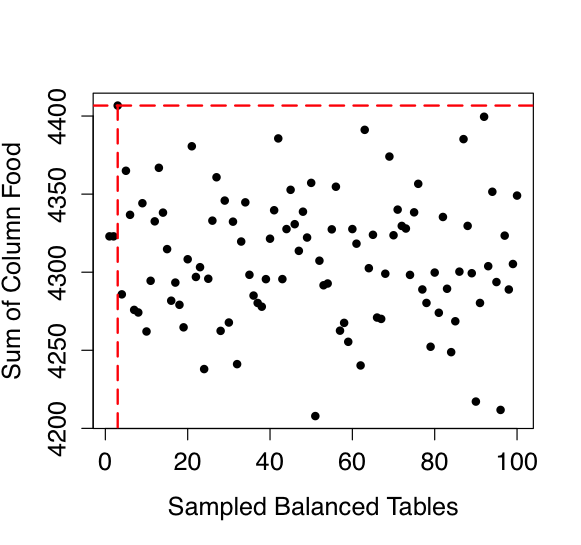
\includegraphics[width=\maxwidth]{figure/ita.png} 
\caption[Total of Food for all sampled tables.]{Total of Food for all sampled tables.
\label{fig:plot}}
\end{center}
\end{figure}
\end{knitrout}


\newpage
In the next table the optimal table, for Italy 2011, is presented


\begin{table}[h!]
  \label{tab:fbs_italy_best}
  \caption{FBS Italy 2011, optimal table}
  \begin{center}
    \begin{tabular}{|c||c|c|c|c|c|c|c|c||c|}
      \hline
       Commodity & Imps & Exps & Feed & Seed & Losses & IndUses & Food & Stock & Prod\\
       \hline\hline
	1. Butter & 21.98 & 3.34 &	0* & 0* & 4.67 & 0 & 40.23 & -6.86 & 33.12\\
       \hline
         2. Barley & 166.04 & 14.82 & 775.24 & 3.88 & 7.58 & 14.35 & 0.12 & 507.76 & 142.19\\
         \hline
         3. Cereals & 13.75 & 1.96 & 2.73 & 0.46 & 1.04 & 2.19 & 1.01 & -16.03 & 11.67\\
         \hline
         \dots  & \dots & \dots & \dots & \dots & \dots & \dots & \dots & \dots & \dots\\
         \hline
         73. Veg & 37.14 & 83.35 & 1.15 & 0* & 1.97 & 0* & 93.21 & 70.64 & 71.90\\
        \hline\hline
        Tot Cols & 4344.18 & 1767.14 & 2881.20 & 126.63 & 379.25 & 342.00 & 4406.70 & 426.15 & 5132.59\\
      \hline
    \end{tabular}
  \end{center}  
\end{table}

Figure \ref{fig:res} shows the variability of the point estimates of Feed in the sampled 
balanced tables. The red dashed lines are the upper and lower bounds reported in Table \ref{tab:fbs_italy_feed}. The blue dashed line is the point estimate of the Feed total given 
by experts, while the red one is the point estimate reported in the "optimal balanced table".

\begin{knitrout}
%\definecolor{shadecolor}{rgb}{0, 0, 0}\color{fgcolor}
\begin{figure}[!ht]
\begin{center}
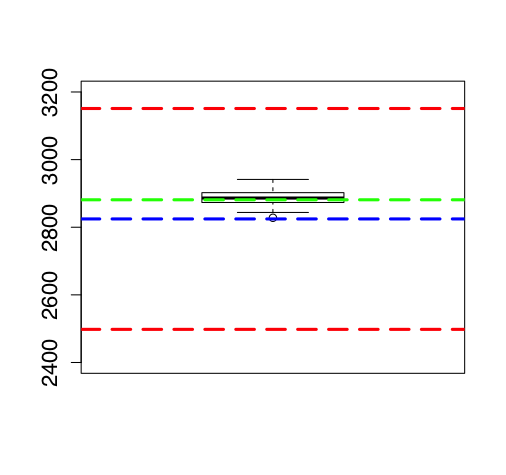
\includegraphics[width=\maxwidth]{figure/res.png} 
\caption[Total of Food for all sampled tables.]{Total of Food for all sampled tables.
\label{fig:plot}}
\end{center}
\end{figure}
\end{knitrout}


\newpage
\section{Conclusions}
The paper shows a flexible algorithm in order to solve the problem of balancing FBS, 
tables measured with uncertainty. The power of this algorithm is in the ability to find 
a solution even in the case of incomplete and unreliable information and allowing the 
user to set several meaningful constrains.
The algorithm is written in the statistical programming language R \cite{rCore} in the 
{\tt constable} package.
For a user friendly tutorial  on conSTable package in Garieri et al., 2015.

\newpage
\section*{Acknowledgement}
This work is supervised by Adam Prakash with assistance from Josef
Schumidhuber, Onno Hoffmeister, Salar Tayyib  whom were crucial in 
the development of the methodology. The author would also like to thank 
the team members which participated in the previous discussions providing 
valuable feedbacks.

\appendix

\section{Supplementary Resources}

The data, source code and documentation can all be found and
downloaded from \url{https://github.com/mrpozzi/conSTable/tree/develop}, the
package can also be installed by following the instruction. 

\FloatBarrier
\section{Pseudo Code}
     

\begin{algorithm}[H]
  \SetAlgoLined
  \KwData{Food Balance Sheet (FBS), Structural Zeros (SZ), Columns Constrains (CC), 
  Objective Function}
  \KwResult{balanced FBS (bFBS)}
  
  \BlankLine
%  Missing values are denoted $\emptyset$\;

  \BlankLine
  Initialization\;
  \Begin{
      \ForAll{cells in i-FBS}{
        Apply structural zeros (i-SZ)
      }
  }  
   
   
  \BlankLine  
  Sampling\;
  \Begin{
      \ForAll{commodities $C_i$}{
          $x_{i.} \leftarrow TN(\mu_{i.},\sigma_{i.}^2)$\\
          $x_{is} \leftarrow R_i - \sum_j^{s-1} x_ij$\\
          \If{$x_{is}$ accetable}{
          continue
          }
       }   
   }

  \BlankLine  
  Constrains and Objective Function\;
  \Begin{
      \ForAll{columns $T_j$}{
          \If{$CC(t_{j,min})\le T_j \le CC(t_{j,max})$)}{
          	add sampled FBS as possible solution
          }
       }
    bFBS $\leftarrow$ OF(all possible FBSs)
   }
   
   
  \caption{Balancing FBS - function
    {\tt conSTable}}
\end{algorithm}

  
  
\begin{thebibliography}{11}
\bibitem{Britz2002}
  Britz W. and Wieck C.,
  \emph{Completeness and Consistency in a Multidimensional Data Base using Constrained Simultaneous Estimation Techniques.},
  2002.
  
\bibitem{Chen2007}
  %Data Collection, Workflows and Methodology (DCWM) team,
  Chen Y. ,
  \emph{Conditional inference on tables with structural zero.},
 Journal of Computational and Graphical Statistics, 16(2), 445-467,
  2007.
  
\bibitem{Chen2005}
  Chen Y., Diaconis P., Holmes S., and Liu J. S.,
  \emph{Sequential Monte Carlo methods for statistical analysis of tables.},
  Journal of the American Statistical Association, 100(469), 109-120,
  2005.
  
\bibitem{Dinwoodie2011}
  Dinwoodie I.H., Chen Y.,
  \emph{Sampling large tables with constrains.},
  Statistica Sinica, 21, 1591-1609,
  2011.
    
\bibitem{Dobra2006}
  Dobra A., Tebaldi C. and West M.,
  \emph{Data augmentation in multi-way contingency tables with fixed marginal totals.} ,
  Journal of Statistical Planning and Inference, 136, 355-372,
  2006.

\bibitem{fao2011}
  FAO
  \emph{Food Balance Sheets: A handbook.} 
  \url{http://www.fao.org/docrep/003/x9892e/x9892e00.htm},
  2011.
 
\bibitem{fao2013}
  FAO, IFAD and WFP,
  \emph{The State of Food Insecurity in the World. The multiple dimensions of food security},
  \url{http://www.fao.org/docrep/018/i3434e/i3434e.pdf},
  2013.
  
\bibitem{fao2014}
  FAO, Statistics Division (ES)
  \emph{A new approach to food balance sheet methods and design.},
  Twenty-fifth Session of the Asia and Pacific Commission on Agricultural Statistics. Ventiane, Lao PDR, February 2014,
  2014.
  
\bibitem{Klaus2014}
  Grunberger K., Statistic Division (ES) FAO
  \emph{Estimating food consumption patterns by reconciling food balance sheets and household budget surveys.},
  Working Paper Series ESS/14-08,
  2014.

\bibitem{Heckelei2008}
 Heckelei T., Mittelhammer R. and Jansson T.,
  \emph{A Bayesian alternative to generalized cross entropy solutions for undeterminated econometric models.},
  Discussion Paper, Institute for Food and Resource Economics,
  2008.
  
\bibitem{Jacobs2002}
  Jacobs K. and Sumner D.A.,
  \emph{The Food Balance Sheets of the Food and Agriculture Organization: a review of potential ways to broden the appropriate uses of the data.},
  FAO Review,
  2002.
  
\bibitem{Mahjoubi2012}
  Mahjoubi R. and Prakash A. ,
  \emph{New framework to compile FAO"s Food Balance Sheets.},
  Twenty-fourth Session of the Asia and Pacific Commission on Agricultural Statistics. Da Lat, Viet Nam,
  2012.
 
 \bibitem{rCore}
  R Core Team,
  \emph{A language and environment for statistical computing.},
  R Foundation for Statistical Computing, Vienna, Austria,
  ISBN 3-900051-07-0, URL http://www.R-project.org/,
  2013.

 
 \bibitem{Robilliard2003}
  Robilliard A.S. and Robinson S.,
  \emph{Reconciling Household Surveys and National Accounts Data using a Cross Entropy Estimation Method.},
  Review of Income and Wealth 49, 395-406,
  2003.
   
 \bibitem{Robinson2000}
  Robinson S., Cattanbo A. and El-Said M,
  \emph{Updating and Estimating a Social Accounting Matrix using Cross Entropy Methods.},
  Economic Systems Research, 13, 47-67,
  2000.
  
   \bibitem{Rodrigues2014}
  Rodrigues J.F.D.,
  \emph{A Bayesian approach to the balancing of sttistical economic data.},
  Entropy, 16, 1243-1271,
  2014.
  
   \bibitem{Tebaldi1998}
  Tebaldi C. and West M.
  \emph{Reconstruction of contingency with missing data.},
  ISDS Discussion Paper, Duke University, n.98-01,
  1998.  
  
  
\end{thebibliography}
  




\end{document}
Status API Training Shop Blog About
� 2015 GitHub, Inc. Terms Privacy Security Contact
%